\documentclass[12pt,a4paper]{article}
\usepackage[utf8]{inputenc}

\title{Filtro crossover} %argomento
\date{17 e 24 aprile, 9 maggio 2024}
\author{Giacomo Errani 1078021 Paolo Forni}

\setlength{\parindent}{20pt}
\usepackage{setspace}
\usepackage[margin=2cm]{geometry}
\usepackage{float}
\usepackage{amsfonts}
\usepackage{pdfpages}
\usepackage{verbatim}
\usepackage[utf8]{inputenc}
\usepackage{subcaption}

\usepackage{graphicx}
\graphicspath{ {./images} } %cartella immagini, separata dalla cartella files

\usepackage{listings}
\usepackage{xcolor}

\definecolor{codegreen}{rgb}{0,0.6,0}
\definecolor{codegray}{rgb}{0.5,0.5,0.5}
\definecolor{codepurple}{rgb}{0.58,0,0.82}
\definecolor{backcolour}{rgb}{0.95,0.95,0.92}

\lstdefinestyle{code_style}{
    backgroundcolor=\color{backcolour},   
    commentstyle=\color{codegreen},
    keywordstyle=\color{magenta},
    numberstyle=\tiny\color{codegray},
    stringstyle=\color{codepurple},
    basicstyle=\ttfamily\footnotesize,
    breakatwhitespace=false,         
    breaklines=true,                 
    captionpos=b,                    
    keepspaces=true,                 
    numbers=left,                    
    numbersep=5pt,                  
    showspaces=false,                
    showstringspaces=false,
    showtabs=false,                  
    tabsize=2
}

\begin{document}

% Some definitions
\newcommand{\theoryF}{ $(1444 \pm 10) \; Hz $}
\newcommand{\amplitudeF}{$(1619 \pm 1) \; Hz $}
\newcommand{\phaseF}{$(1437 \pm 2) \; Hz $}

\maketitle

\section{Abstract}

\indent In questo esperimento abbiamo ricreato un filtro crossover a due canali e ne abbiamo analizzato il comportamento in risposta ad un'onda sinusoidale. Analizzando la variazione dell'ampiezza dei segnali sui canali Tweeter e Woofer abbiamo ottenuto la frequenza di cross pari a \amplitudeF. Analizzando lo sfasamento relativo, abbiamo ottenuto la frequenza \phaseF. E' stato inoltre calcolato il valore atteso \theoryF \hspace{1pt} mediante misura diretta dell'induttanza sul ramo del Woofer e della capacità sul ramo del Tweeter. 

La frequenza ottenuta a partire dallo sfasamento è risultata compatibile con il valore teorico atteso, mentre quella ottenuta a partire dall'ampiezza no (per ora :( ).

\section{Introduzione}
Il filtro crossover è un circuito RLC costituito da due rami: uno con un filtro passa basso realizzato mediante un induttore e una resistenza in serie, l'altro un filtro passa alto realizzato mediante condensatore e resistenza in seri

\section{Apparato sperimentale}

\begin{figure}[H]
\centering
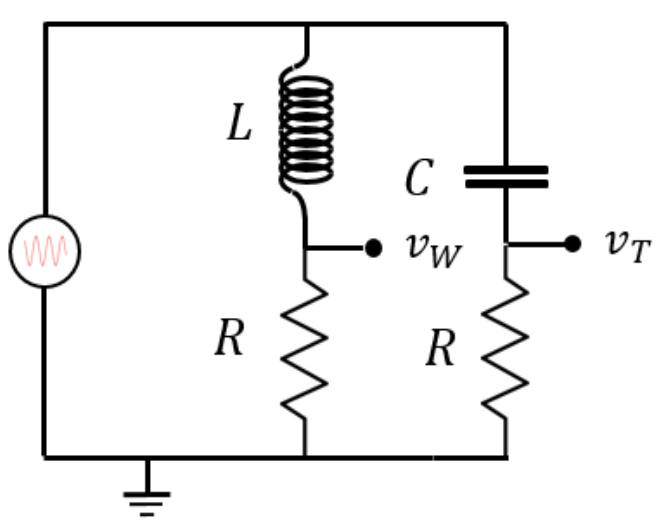
\includegraphics[width=8cm]{crossover_scheme.png}

\caption{Schema del circuito}
\label{Fig1}

\end{figure}

e (Figura \ref{Fig1}).



\section{Analisi}

\subsection{Analisi preliminare qualitativa}

\subsection{Analisi della frequenza misurata}

\subsection{Analisi dell'ampiezza}

\subsection{Analisi della fase}

\section{Appendice}

\subsection{Formule e dimostrazioni}

\subsection{Correzione dettagliata errori sistematici}



\end{document}
